\PassOptionsToPackage{table,xcdraw}{xcolor}
\documentclass[dvipsnames]{rvexam}

%\numofcos{3x}
%%%%%%%%%%%%%%%%%%%%%Packages%%%%%%%%%%%%%%%%%%
\usepackage{tikz}
\usetikzlibrary{shapes,snakes}
\usepackage[american voltages, american currents,siunitx]{circuitikz}
\usetikzlibrary{circuits.logic.US} 
\ctikzset{tripoles/mos style/arrows}
\ctikzset{tripoles/pmos style/emptycircle}
\usetikzlibrary{decorations.text}%For text along the path
\usetikzlibrary{intersections,calc,backgrounds}
\usetikzlibrary{patterns}

%%Tikz Graphs based
\usepackage{pgfplots}
\usetikzlibrary{pgfplots.groupplots}%for multiplot
\usepackage[miktex]{gnuplottex}
\usetikzlibrary{arrows}
\usepackage{tikz-timing}
\usetikztiminglibrary{overlays}%for overlap of 2 or more waves
\usetikztiminglibrary{advnodes-cfr}%for using center of an edge
%for removing the error while introducing \\ in text
%%Others
\usepackage{karnaughmap}[2013/12/06]

\usepackage{cancel}
%\usepackage[utf8]{inputenc}
\usepackage{float}
%\usepackage[demo]{graphicx}
\usepackage{subcaption}
\usepackage{sidecap}%For side captions

\usepackage{comment}
\usepackage{amsmath}
\usepackage{amssymb}
\usepackage{enumerate}

\usepackage{siunitx}

\usepackage[hidelinks]{hyperref}
%\usepackage{fancyhdr}
\usepackage{tabularx}

%\usepackage{booktabs}
%\usepackage{multirow}
%\usepackage{multicol}
%\usepackage{makecell}

\usepackage[most]{tcolorbox}
%Boxed text using "tcolorbox"
\usepackage{varwidth}

\usepackage{xcolor}
\usepackage{color} % defines a new color
\shadedsolutions % defines the style of the solution environment
\definecolor{SolutionColor}{rgb}{0.95,0.95,0.95} % light blue

% \framedsolutions % defines the style of the solution environment
% Defines the title of the solution environment:
\renewcommand{\solutiontitle}{\noindent\textbf{Solution:}\par\noindent}

%%%%%%%%%%%%%%%%%%%%Macros%%%%%%%%%%%%%%%%%%%%
\newcommand*{\myparse}[2][sci,precision=2]{%
  \pgfkeys{/pgf/fpu}%
  \pgfmathparse{#2}%
  \pgfmathprintnumber[#1]{\pgfmathresult}%
  \pgfkeys{/pgf/fpu=false}%
}

\makeatletter
\long\def\ifnodedefined#1#2#3{%
    \@ifundefined{pgf@sh@ns@#1}{#3}{#2}%
}
\makeatother

%Used to hide/show questions
\newif\ifsee \seefalse

\newif\ifkeepquestion \keepquestiontrue
\NewEnviron{qsn}{\ifkeepquestion\BODY\fi}

\newif\ifshortans \shortanstrue
\NewEnviron{shortanswer}{\ifshortans\BODY\fi}

\newif\iflongans \longansfalse
\NewEnviron{longanswer}{\iflongans\BODY\fi}
%%%%%%%%%%%%%%%%%%%%%%%%%%%%%%%%%%%%%%%%%%%%%
\printanswers %Used to print the answers
%\noprintanswers
\keepquestiontrue
\shortanstrue
\longansfalse
\seefalse
%%%%%%%%%%%%%%%%%%%%%%%%%%%%%%%%%%%%%%%%%%%%%%
\title{AICD Test 3}
\author{P Narashimaraja }
\gdef\date{Jul 2021}

\gdef\courseTitle{Analog IC Design}
\gdef\courseCode{18EC46}
\gdef\sem{IV}
\ifsee{}\else
\gdef\testTitle{Re-Test - 3} \fi
%%%%%%%%%%%%%%%%%%%%%%%%%%%%%%%%%%%%%%%%%%%%%%%

\ifkeepquestion{
%Header
\gdef\lftfp{\includegraphics[width=1.5cm]{Figs/RVCE_logo}}
\gdef\midfp{
\large\textbf{R.V.COLLEGE OF ENGINEERING, Bengaluru - 59}\\
\normalsize\textbf{Department of Electronics \& Communication Engineering}\\
\normalsize{\href{www.rvce.edu.in}{www.rvce.edu.in} ; \href{mailto://hod.ec@rvce.edu.in}{hod.ec@rvce.edu.in} ; +91-9900700990 ; 080-6717 8042}
}
\gdef\ritfp{}

\gdef\lftrp{}
\gdef\midrp{}
\gdef\ritrp{\date}

%Footer
\gdef\@footrit{\thepage$\vert$\numpages}

}\else{
\gdef\lftfp{.\\
\small\textbf{COURSE CODE:}\courseCode}
\gdef\midfp{\small\textbf{SCHEME \& SOLUTION}\\
\small\textbf{\qquad\qquad\;  COURSE:} \courseTitle}
\gdef\ritfp{\date\\
UG}

\gdef\lftrp{.\\
\small\textbf{COURSE CODE:}\courseCode}
\gdef\midrp{\small\textbf{SCHEME \& SOLUTION}\\
\small\textbf{\qquad\qquad\;  COURSE:} \courseTitle}
\gdef\ritrp{\date\\
UG}

%Footer
\gdef\@footrit{\thepage/\numpages}
}
\fi

\pagestyle{headandfoot}
\runningheadrule

\firstpageheader{\leavevmode\lftfp}{\leavevmode\midfp}{\leavevmode\ritfp}
\runningheader{\leavevmode\lftrp}{\leavevmode\midrp}{\leavevmode\ritrp}

\firstpagefooter{}{}{\leavevmode\@footrit}
\runningfooter{}{}{\leavevmode\@footrit}
 
%For bookmarking the questions
\hypersetup{
    pdftitle={AICD Test 1},
    pdfauthor={P Narashimaraja},
    pdfsubject={AICD 18EC46},
%    pdfkeywords={keyword1, keyword2},
    bookmarksnumbered=true,     
    bookmarksopen=true,         
    bookmarksopenlevel=1,       
    colorlinks=false,            
    pdfstartview=FitH,           
    pdfpagemode=UseOutlines,    % this is the option you were lookin for
    pdfpagelayout=OneColumn
}

\begin{document}

\ifsee{
%\maketitle
}\else{
\begin{center}
\sem\; Semester  \par
\testTitle   \par
\end{center}

\begin{minipage}[t]{10cm}
\flushleft
\textbf{Course: \courseTitle}\par
\textbf{Time: 1.5 Hours} \par
\end{minipage}
\hfill
\begin{minipage}[t]{5cm}
\flushright
\textbf{Course Code: \courseCode}\par
\textit{Max Marks: 50}
\end{minipage}
}
\fi
\vspace{0.2cm}
%\textbf{Instructions to candidates:} Answer all the questions.\\ 
\vspace{2mm}
%\begin{tabularx}{\textwidth}{p{15cm} X} 
%	\centerline{\textsc{Part a}} &  
%\end{tabularx}

\begin{questions}
%\pointsinleftmargin
%\pointsinrightmargin
\pointsdroppedatright
\addpoints 
%1
\question
\begin{parts}
\part[5][1][1]
\xdef\Fo{(10*pow(10,3))}
\xdef\Q{2}
\xdef\C{(1*pow(10,-9))}
Assuming ideal opamp, determine the transfer function of KHN biquad high pass filter. Design a KHN circuit to realize a high pass function with $f_{o}=\myparse[fixed]{\Fo*pow(10,-3)} KHz$ and $Q = \Q$, assume the integrators have same resistors and capacitors, with $C=\myparse[fixed]{\C*pow(10,9)}nF$. What is the value of high frequency gain obtained? What is the centre frequency gain of bandpass function that is simultaneously available at the output of the first integrator? 
%\droppoints

\begin{solution}
\begin{equation}
\begin{split}
\dfrac{V_{out}}{V_{in}}(S)&=\dfrac{b_{2}S^{2}}{S^{2}+\dfrac{\omega_{n}}{Q}S+\omega_{n}^{2}}\\
V_{out}(S)&= b_{2}V_{in}(S)-\dfrac{\omega_{n}}{Q}\dfrac{1}{S}V_{out}(S)-\dfrac{\omega^{2}_{n}}{S^{2}}V_{out}(S)
\end{split}\tag{1M}
\end{equation}

\end{solution}

\part[5][3][3]
fl;kajs \droppoints
\end{parts}

\question[10][3][4]
\xdef\Fo{(10*pow(10,3))}
\xdef\Q{2}
\xdef\C{(1*pow(10,-9))}
Assuming ideal opamp, determine the transfer function of KHN biquad high pass filter. Design a KHN circuit to realize a high pass function with $f_{o}=\myparse[fixed]{\Fo*pow(10,-3)} KHz$ and $Q = \Q$, assume the integrators have same resistors and capacitors, with $C=\myparse[fixed]{\C*pow(10,9)}nF$. What is the value of high frequency gain obtained? What is the centre frequency gain of bandpass function that is simultaneously available at the output of the first integrator? 
\droppoints

\question
\begin{parts}
\part[7][2][6]
%a
\xdef\Vdd{3}
\xdef\Kn{(36*pow(10,-5))}
\xdef\Kp{(9*pow(10,-5))}
\xdef\VTn{0.7}
\xdef\VTp{0.8}
\xdef\WLa{(50/0.5)}
\xdef\WLb{(72/0.5)}
\xdef\Iss{(1*pow(10,-3))}
\xdef\Io{(0.5*pow(10,-3))}
\xdef\lmbn{0.1}
\xdef\lmbp{0.1}
In the two-stage op-amp of Fig.a, $(W/L)=\WLa$ for all transistors except for $M_{5}$, for which $(W/L)_{5}=\WLb$. Also, $I_{D7}=\myparse[fixed]{\Iss*pow(10,3)} mA$ and the output branch is biased at $\myparse[fixed]{\Io*pow(10,3)} mA$. Given $V_{DD}=\Vdd V, K^{'}_{n}=\myparse[fixed]{\Kn*pow(10,6)}\mu A/V^{2}, K^{'}_{p}=\myparse[fixed]{\Kp*pow(10,6)}\mu A/V^{2}, \lambda_{n}=\lmbn V^{-1}, \lambda_{p}=\lmbp V^{-1}, V_{Tn}=\VTn V$ and $V_{Tp}=-\VTp V$.
\begin{enumerate}[i.]
\item Determine the CM level at nodes X and Y.
\item Calculate the maximum output voltage swing.
\item Calculate the total gain of the op-amp.
\end{enumerate}
\droppoints
 
\begin{figure}[H]
\begin{subfigure}[b]{0.5\textwidth}
\centering
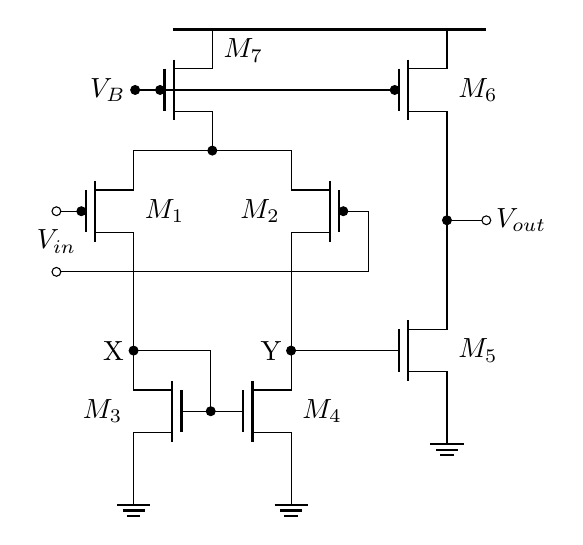
\begin{tikzpicture}
\draw(0,0)node[ground](gnd){}node[nmos, anchor=S, xscale=-1](m3){}++(2,0)node[ground]{}node[nmos, anchor=S, xscale=1](m4){}
	(m3.D)node[circ]{}-|(m3.G)node[circ]{}to(m4.G)
	(m3.D)node[left]{X}to++(0,1)node[pmos, anchor=D](m1){}
	(m4.D)node[left]{Y}node[circ]{}to++(0,1)node[pmos, anchor=D, xscale=-1](m2){}
	(m1.S)to(m2.S)
	($(m1.S)!0.5!(m2.S)$)node[circ](vp){}node[pmos, anchor=D](m7){}
	
	(m4.D)to++(1,0)node[nmos, anchor=G](m5){}
	(m5.S)node[ground]{}
	(m5.D|-m7.D)node[pmos, anchor=D](m6){}
	(m5.D)to(m6.D)
	($(m5.D)!0.5!(m6.D)$)node[circ](vo){}to++(0.5,0)node[ocirc]{}node[right]{$V_{out}$}
	
	(m6.G)to(m7.G)node[circ]{}node[left]{$V_{B}$}
	(m2.G)to(m2.G|-m2.D)to(m1.G|-m1.D)node[ocirc]{}
	($(m1.G)!0.5!(m1.G|-m1.D)$)node{$V_{in}$}
	(m1.G)node[ocirc]{}
	(m4.G)++(1,0)node[right]{$M_{4}$}
	(m1.G)++(1,0)node[right]{$M_{1}$}
	(m3.G)++(-1,0)node[left]{$M_{3}$}
	(m2.G)++(-1,0)node[left]{$M_{2}$}
	(m5.G)++(1,0)node[right]{$M_{5}$}
	(m6.G)++(1,0)node[right]{$M_{6}$}
	(m7.G)++(1,0.5)node[right]{$M_{7}$}
	;
\draw[very thick](m7.S)++(-0.5,0)to($(m6.S)+(0.5,0)$);
\end{tikzpicture}
\caption*{Fig.a}
\end{subfigure}
%
\begin{subfigure}[b]{0.5\textwidth}
\centering
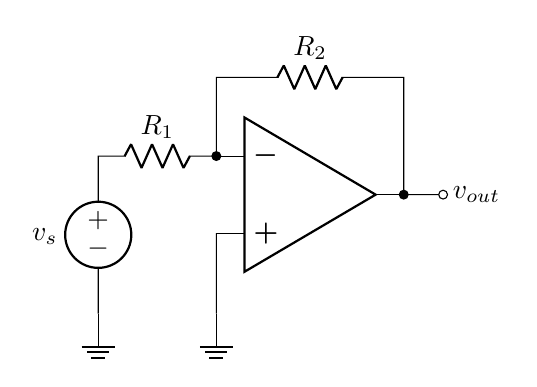
\begin{tikzpicture}
\draw(0,0)node[ground](gnd){}to [V,l=$v_{s}$, invert]++(0,2)to[R,l=$R_{1}$,/tikz/circuitikz/bipoles/length=1cm]++(1.5,0)node[circ](vm){}node[op amp, anchor=-, yscale=1](op){}
	(vm.center)to++(0,1)node(vm2){}to[R,l=$R_{2}$,/tikz/circuitikz/bipoles/length=1cm](vm2-|op.out)to(op.out)node[circ](out){}to++(0.5,0)node[ocirc](out2){}node[right]{$v_{out}$}
	(op.+)node(vp){}to(vp|-gnd)node[ground]{}
	;
\end{tikzpicture}
\caption*{Fig.b}
\end{subfigure}
\end{figure}

%b
\part[3][3][2]
\xdef\bta{0.75}
\xdef\gerr{0.01}
\xdef\Ra{(1*pow(10,3))}
\pgfmathparse{(\bta/(1-\bta))}\xdef\Acl{\pgfmathresult}
If the above op-amp is used in a closed loop configuration (as shown in Fig.b) with $R_{1}=\myparse[fixed]{\Ra*pow(10,-3)} k\Omega$ to achieve a closed-loop DC gain of $-\myparse[fixed]{(\bta/(1-\bta))}\xdef\Acl{\pgfmathresult}$, calculate the value of $R_{2}$ that is required to achieve the required closed-loop gain and the gain error that results due to finite open-loop gain.
\droppoints

\end{parts}
\end{questions}

\cobttable
%\vspace{1cm}
%\begin{table}[H]
%\centering
%\begin{tabular}{|c|c|c|c|c|c|c|c|c|c|c|c|c|}
% \multicolumn{13}{c}{BT-Blooms Taxonomy; CO-Course Outcomes; M-Marks}\\
%\hline
%\multirow{2}{*}{\makecell{\vspace{0.1cm}\\ Marks \\ Distribution}}& \multicolumn{2}{c|}{Particulars}& CO1 & CO2 & CO3 & CO4 & L1 & L2 & L3 & L4 & L5 & L6\\ \cline{2-13}
%&Test & \makecell{Max \\ Marks} &20 &14 &10 &6 &15 &25 &6 &4 &- &-\\ 
%\hline
%\end{tabular}
%\end{table}
\end{document}
